% Options for packages loaded elsewhere
\PassOptionsToPackage{unicode}{hyperref}
\PassOptionsToPackage{hyphens}{url}
%
\documentclass[
]{article}
\usepackage{amsmath,amssymb}
\usepackage{lmodern}
\usepackage{iftex}
\ifPDFTeX
  \usepackage[T1]{fontenc}
  \usepackage[utf8]{inputenc}
  \usepackage{textcomp} % provide euro and other symbols
\else % if luatex or xetex
  \usepackage{unicode-math}
  \defaultfontfeatures{Scale=MatchLowercase}
  \defaultfontfeatures[\rmfamily]{Ligatures=TeX,Scale=1}
\fi
% Use upquote if available, for straight quotes in verbatim environments
\IfFileExists{upquote.sty}{\usepackage{upquote}}{}
\IfFileExists{microtype.sty}{% use microtype if available
  \usepackage[]{microtype}
  \UseMicrotypeSet[protrusion]{basicmath} % disable protrusion for tt fonts
}{}
\makeatletter
\@ifundefined{KOMAClassName}{% if non-KOMA class
  \IfFileExists{parskip.sty}{%
    \usepackage{parskip}
  }{% else
    \setlength{\parindent}{0pt}
    \setlength{\parskip}{6pt plus 2pt minus 1pt}}
}{% if KOMA class
  \KOMAoptions{parskip=half}}
\makeatother
\usepackage{xcolor}
\usepackage[margin=1in]{geometry}
\usepackage{longtable,booktabs,array}
\usepackage{calc} % for calculating minipage widths
% Correct order of tables after \paragraph or \subparagraph
\usepackage{etoolbox}
\makeatletter
\patchcmd\longtable{\par}{\if@noskipsec\mbox{}\fi\par}{}{}
\makeatother
% Allow footnotes in longtable head/foot
\IfFileExists{footnotehyper.sty}{\usepackage{footnotehyper}}{\usepackage{footnote}}
\makesavenoteenv{longtable}
\usepackage{graphicx}
\makeatletter
\def\maxwidth{\ifdim\Gin@nat@width>\linewidth\linewidth\else\Gin@nat@width\fi}
\def\maxheight{\ifdim\Gin@nat@height>\textheight\textheight\else\Gin@nat@height\fi}
\makeatother
% Scale images if necessary, so that they will not overflow the page
% margins by default, and it is still possible to overwrite the defaults
% using explicit options in \includegraphics[width, height, ...]{}
\setkeys{Gin}{width=\maxwidth,height=\maxheight,keepaspectratio}
% Set default figure placement to htbp
\makeatletter
\def\fps@figure{htbp}
\makeatother
\setlength{\emergencystretch}{3em} % prevent overfull lines
\providecommand{\tightlist}{%
  \setlength{\itemsep}{0pt}\setlength{\parskip}{0pt}}
\setcounter{secnumdepth}{-\maxdimen} % remove section numbering
\ifLuaTeX
  \usepackage{selnolig}  % disable illegal ligatures
\fi
\IfFileExists{bookmark.sty}{\usepackage{bookmark}}{\usepackage{hyperref}}
\IfFileExists{xurl.sty}{\usepackage{xurl}}{} % add URL line breaks if available
\urlstyle{same} % disable monospaced font for URLs
\hypersetup{
  pdftitle={Analysis of College Majors and Impact on Employment},
  pdfauthor={Arona Cho, Irene Jo, Melanie Kuo},
  hidelinks,
  pdfcreator={LaTeX via pandoc}}

\title{Analysis of College Majors and Impact on Employment}
\author{Arona Cho, Irene Jo, Melanie Kuo}
\date{11/13/2022}

\begin{document}
\maketitle

\hypertarget{abstract}{%
\subsubsection{Abstract:}\label{abstract}}

Our main concern for this project is to find the relationships between
various college majors, employment and salary as well as graduation
rates. This is important information since this can be used to further
predict future supply of workers in various fields as well as the
demands of various job fields. To address this, we will provide large
amounts of data on employment and unemployment rates, median salary,
number of graduates and gender distribution across 173 college majors
surveyed in the American Community Survey 2010-2012 Public Use Microdata
Series.

\hypertarget{keywords}{%
\subsubsection{Keywords:}\label{keywords}}

College majors, employment, unemployment, salary, age/gender

\hypertarget{introduction}{%
\subsubsection{Introduction:}\label{introduction}}

For our project, we are analyzing hundreds of different college majors
and their correlation to employment and unemployment. The categories we
analyze are divided by age (all ages, under 28, and over 25), and we
also will take a look at basic earnings and sex. Our goal is to
determine whether or not one's major has any impact on their future
employment. The FiveThirtyEight article ``The Economic Guide to Picking
a Major'' uses this dataset to demonstrate the importance behind picking
a major: ``A college degree is no guarantee of economic success. But
through their choice of major, they can take at least some steps toward
boosting their odds'' (Casselman). We want to assess if majors are truly
as important as perceived, and if majoring in something that may be
perceived to have a low or high employment rate may actually turn out to
have a different or unexpected outcome.

\hypertarget{problem-domain}{%
\subsubsection{Problem Domain:}\label{problem-domain}}

Our project frame is finding employment and unemployment rates as well
as rates of graduation and gender distribution within the 173 majors.
With this information, we hope to discover various trends and patterns
that can be further utilized to predict future job market changes as
well as to inform students tasked with making decisions that will have
long lasting effects in their lives.

The human values that we took into consideration while working on this
project were the long term effects of making these conclusions from this
data collected in American Community Survey 2010-2012, as we could end
up discouraging some people from certain job fields and causing a shift
in supply of certain college major graduates in the job field. To avoid
spreading inaccurate information, we made sure to draw accurate
conclusions from reliable and quantitative data and utilizing analytic
methods to make accurate conclusions.

Direct stakeholders of this project include us, the authors, as we would
like to make sure it includes accurate, reliable, and useful
information. If we cannot deliver information that does not meet those
requirements, then we would fail to meet our objective of assessing the
importance of the type of college major in relation to other factors
such as employment rate and gender distribution. Other direct
stakeholders for this project are the future and current college
enrollees that would benefit from our assessment of college majors. The
Federal Reserve Bank of New York reported that there is currently a
growing wage gap between those without a college degree and those with a
college degree (The Federal Reserve Bank of New York). People that
consider income to be crucial to their choice of major would be one of
the main stakeholders of this project. Possible indirect stakeholders
could be the institutions that facilitate and educate people that would
like to pursue college degrees, as well as employers and the fields of
the different majors listed in this project.

Possible harms of this project include biases and reinforcement of
stereotypes that may be formed regarding specific majors. Through the
analysis of this project, there may be data conclusions that are
unexpected, such as seemingly high-paying majors not paying as much, or
vice versa. The analysis of this data could possibly affect one's
decision of what to major in college, which can be both a harm or
benefit. One may choose a specific major due to factors like income or
employment rates, so this information can be useful to some, and may
provide benefits by assisting with these types of decisions. It's also
important to know information regarding the amount of women in certain
fields in order to assess areas where more gender diversity is needed.
According to the National Girls Collaborative Project, women make up
only 34\% of the STEM workforce (National Girls Collaborative Project).
This means that many progressions need to be made towards closing the
gender gap, and using this data is a great start.

\hypertarget{research-questions}{%
\subsubsection{Research Questions}\label{research-questions}}

\hypertarget{what-are-the-median-wages-of-college-graduates-with-different-majors}{%
\paragraph{\texorpdfstring{\emph{What are the median wages of college
graduates with different
majors?}}{What are the median wages of college graduates with different majors?}}\label{what-are-the-median-wages-of-college-graduates-with-different-majors}}

Finding the median wages of college graduates with various majors can
help students get a better understanding of levels of financial success
of graduates with different majors and help them make a decision that
best matches their dreams. It can also be used for those in specific
majors to estimate their future wage and calculate their financial
status.

\hypertarget{which-college-majors-result-in-higher-rates-of-employment-and-salary}{%
\paragraph{\texorpdfstring{\emph{Which college majors result in higher
rates of employment and
salary?}}{Which college majors result in higher rates of employment and salary?}}\label{which-college-majors-result-in-higher-rates-of-employment-and-salary}}

This data helps identify different patterns in growing and shrinking
fields of study to be used to further predict the job market changes as
well as assist students that have to choose a major by providing
important information of employment and salary rates.

\hypertarget{what-are-the-relationships-between-gender-and-college-majors}{%
\paragraph{\texorpdfstring{\emph{What are the relationships between
gender and college
majors?}}{What are the relationships between gender and college majors?}}\label{what-are-the-relationships-between-gender-and-college-majors}}

This information is important since it helps data about gender
inequality and distribution amongst the different majors easier to view
and understand. This allows us to discover which majors are preferred by
different genders and possibly carry on further research about why.

\hypertarget{how-do-the-graduation-rates-of-each-major-compare-to-others}{%
\paragraph{\texorpdfstring{\emph{How do the graduation rates of each
major compare to
others?}}{How do the graduation rates of each major compare to others?}}\label{how-do-the-graduation-rates-of-each-major-compare-to-others}}

It is important because it can be informative for those going into the
major and those that are choosing majors to take into consideration the
rates of graduation based on academic rigor, lack of employment offers
or overall bad staff. This information is needed to help the school make
improvements or assistance for students in majors with very low
graduation rates or etc.

\hypertarget{the-dataset}{%
\subsubsection{The Dataset}\label{the-dataset}}

Our dataset showcases information regarding various majors and their
statistics for employment, graduation rates, and gender. From viewing
this dataset, we can identify correlations between the data, and
determine whether or not these factors have impacts on one another.
Additionally, the dataset has a vast amount of information, which is
useful for those who may be interested in finding a less popular major
or specific, researched statistics regarding another specific major.

\begin{center}\rule{0.5\linewidth}{0.5pt}\end{center}

\hypertarget{table-1.-summary-of-the-dataset.}{%
\subparagraph{Table 1. Summary of the
dataset.}\label{table-1.-summary-of-the-dataset.}}

\begin{longtable}[]{@{}lll@{}}
\toprule()
Data File & Num of observations (row) & Num of var (col) \\
\midrule()
\endhead
All-ages & 173 & 10 \\
Grad-students & 173 & 10 \\
Majors-list & 174 & 3 \\
Recent-grades & 173 & 10 \\
Women-stem & 76 & 9 \\
\bottomrule()
\end{longtable}

Tunguz, Bojan. All-ages (Data set), 2020.

\url{https://www.kaggle.com/datasets/tunguz/college-majors?select=all-ages.csv}

Tunguz, Bojan. Grad-students (Data set), 2020.

\url{https://www.kaggle.com/datasets/tunguz/college-majors?select=grad-students.csv}

Tunguz, Bojan. Majors-list (Data set), 2020.

\url{https://www.kaggle.com/datasets/tunguz/college-majors?select=majors-list.csv}

Tunguz, Bojan. Recent-grads (Data set), 2020.

\url{https://www.kaggle.com/datasets/tunguz/college-majors?select=recent-grads.csv}

Tunguz, Bojan. Women-stem (Data set), 2020.

\url{https://www.kaggle.com/datasets/tunguz/college-majors?select=women-stem.csv}

\hypertarget{provenance}{%
\subsubsection{Provenance}\label{provenance}}

This data was collected in 2020 by Bojan Tunguz, a data scientist from
Indiana. While there is little information regarding the purpose behind
the collection of the dataset, Tunguz has compiled hundreds of datasets
regarding a wide variety of topics and has an extremely high ranking
with Kaggle, and one can infer that his purpose behind this data
collection was pure interest regarding the topic at hand. Tunguz used
the American County Survey 2010-2012 for statistics behind these majors.

The data collection effort of the American County Survey of 2010-2012
was federally funded as the data was obtained from the U.S. Census. For
Tunguz, they were able to collect the data through public sources as
listed on the U.S. Census Bureau website. Those that have an interest in
a specific major's post-graduate employment rate would most likely
benefit from this data. Financially, people who are researching for the
purpose of finding which major would have the highest employment rate
for their career would most likely benefit.

The data was validated and held secure by its source of collection,
which is the U.S. Census Bureau. The residents that complete the survey
are required by law to accurately respond, while the U.S. Census Bureau
is held by the law to keep the information confidential. As it is a
government survey, it is held as a credible source as it should be an
accurate reflection of the state of residents of the United States.
However, due to the census data being self-reported, there may be
response bias present in the data.

Through Kaggle, a platform that allows for the publishing and sharing of
datasets, we searched for datasets regarding college majors as our key
interest. Through there, we found this dataset and found the contents of
it interesting as it specifically included the statistics of women in
STEM. As all three of us are women in STEM, we decided to choose this
dataset because of its relevance to our personal career goals and
aspirations. We do credit the source of the data, Bojan Tunguz, by the
citations done above.

\hypertarget{acknowledgements}{%
\subsubsection{Acknowledgements}\label{acknowledgements}}

Thank you to our TA for helping out with these assignments :)

\hypertarget{references}{%
\subsubsection{References}\label{references}}

Bencasselman. ``The Economic Guide to Picking a College Major.''
FiveThirtyEight, FiveThirtyEight, 12 Sept.~2014,
\url{https://fivethirtyeight.com/features/the-economic-guide-to-picking-a-college-major/}.

``The Labor Market for Recent College Graduates.'' Federal Reserve Bank
of New York, 2021,
\url{https://www.newyorkfed.org/research/college-labor-market/college-labor-market_wages.html}

``State of Girls and Women in Stem.'' National Girls Collaborative
Project, 28 February 2022,
\url{https://ngcproject.org/resources/state-girls-and-women-stem}.

\hypertarget{dynamic-paragraph}{%
\subsubsection{Dynamic Paragraph}\label{dynamic-paragraph}}

We determined the median earnings of full-time, year-round workers of
those in the \texttt{women-stem.csv} file. This data was evaluated for
the purpose of determining what salaries women earned. The max median
earning was list(Median = 110000), while the minimum median earnings as
list(Median = 26000). The average of the salaries was 46118.4210526316,
and median between the observations was 44350. Lastly, we also
calculated the range of the observations, which was 84000.

\hypertarget{b.3-table}{%
\subsubsection{B.3 \textbar{} Table}\label{b.3-table}}

\begin{verbatim}
##          Major Catagories Total Number of Women
## 1  Biology & Life Science             19210.214
## 2 Computers & Mathematics              8207.545
## 3             Engineering              4457.793
## 4                  Health             32309.417
## 5       Physical Sciences              9008.900
\end{verbatim}

Our data table demonstrated the total number of women in different major
categories, analyzing which categories had the highest and lowest
percentages of women with an emphasis on the study of STEM categories.
While the ``Health'' category had the highest amount of women, the data
indicated a drastic lack in the number of women in the ``Computers \&
Mathematics'' fields, as well as the ``Engineering'' field. This
demonstrated that a lack of gender diversity is prominent in
technological fields, such as Computer Science \& Mathematics and
Engineering.

\hypertarget{b.4-shares-of-total-women-in-stem-majors}{%
\subsubsection{B.4 \textbar{} Shares of Total Women in STEM
Majors}\label{b.4-shares-of-total-women-in-stem-majors}}

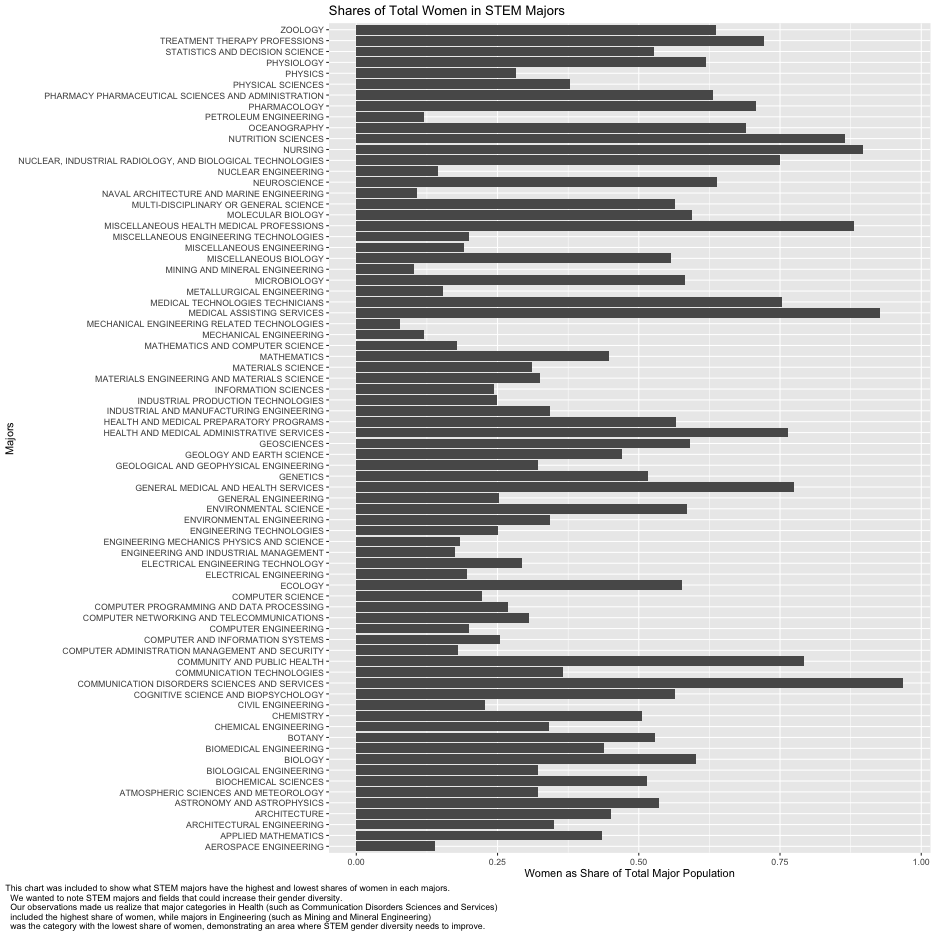
\includegraphics{index_files/figure-latex/womenstem-1.pdf} This chart
was included to show what STEM majors have the highest and lowest shares
of women in each majors. We wanted to note STEM majors and fields that
could increase their gender diversity. Our observations made us realize
that major categories in Health (such as Communication Disorders
Sciences and Services) included the highest share of women, while majors
in Engineering (such as Mining and Mineral Engineering) was the category
with the lowest share of women, demonstrating an area where STEM gender
diversity needs to improve.

\hypertarget{b.5-major-list-treemap}{%
\subsubsection{B.5 \textbar{} Major List
Treemap}\label{b.5-major-list-treemap}}

\begin{verbatim}
## $tm
##                                  group                            subgroup
## 1      Agriculture & Natural Resources     Agriculture & Natural Resources
## 2      Agriculture & Natural Resources                                <NA>
## 3                                 Arts                                Arts
## 4                                 Arts                                <NA>
## 5               Biology & Life Science              Biology & Life Science
## 6               Biology & Life Science                                <NA>
## 7                             Business                            Business
## 8                             Business                                <NA>
## 9          Communications & Journalism         Communications & Journalism
## 10         Communications & Journalism                                <NA>
## 11             Computers & Mathematics             Computers & Mathematics
## 12             Computers & Mathematics                                <NA>
## 13                           Education                           Education
## 14                           Education                                <NA>
## 15                         Engineering                         Engineering
## 16                         Engineering                                <NA>
## 17                              Health                              Health
## 18                              Health                                <NA>
## 19           Humanities & Liberal Arts           Humanities & Liberal Arts
## 20           Humanities & Liberal Arts                                <NA>
## 21 Industrial Arts & Consumer Services Industrial Arts & Consumer Services
## 22 Industrial Arts & Consumer Services                                <NA>
## 23                   Interdisciplinary                   Interdisciplinary
## 24                   Interdisciplinary                                <NA>
## 25                 Law & Public Policy                 Law & Public Policy
## 26                 Law & Public Policy                                <NA>
## 27         Less than Bachelor's Degree         Less than Bachelor's Degree
## 28         Less than Bachelor's Degree                                <NA>
## 29                   Physical Sciences                                <NA>
## 30                   Physical Sciences                   Physical Sciences
## 31            Psychology & Social Work                                <NA>
## 32            Psychology & Social Work            Psychology & Social Work
## 33                      Social Science                                <NA>
## 34                      Social Science                      Social Science
##    vSize vColor stdErr vColorValue level        x0         y0          w
## 1     10      1     10          NA     2 0.7947455 0.72000000 0.20525452
## 2     10      1     10          NA     1 0.7947455 0.72000000 0.20525452
## 3      8      1      8          NA     2 0.5689655 0.00000000 0.20935961
## 4      8      1      8          NA     1 0.5689655 0.00000000 0.20935961
## 5     14      1     14          NA     2 0.3448276 0.64102564 0.22413793
## 6     14      1     14          NA     1 0.3448276 0.64102564 0.22413793
## 7     13      1     13          NA     2 0.3448276 0.30769231 0.22413793
## 8     13      1     13          NA     1 0.3448276 0.30769231 0.22413793
## 9      4      1      4          NA     2 0.7783251 0.00000000 0.14778325
## 10     4      1      4          NA     1 0.7783251 0.00000000 0.14778325
## 11    11      1     11          NA     2 0.5689655 0.72000000 0.22577997
## 12    11      1     11          NA     1 0.5689655 0.72000000 0.22577997
## 13    16      1     16          NA     2 0.0000000 0.00000000 0.17797553
## 14    16      1     16          NA     1 0.0000000 0.00000000 0.17797553
## 15    29      1     29          NA     2 0.0000000 0.51666667 0.34482759
## 16    29      1     29          NA     1 0.0000000 0.51666667 0.34482759
## 17    12      1     12          NA     2 0.3448276 0.00000000 0.22413793
## 18    12      1     12          NA     1 0.3448276 0.00000000 0.22413793
## 19    15      1     15          NA     2 0.1779755 0.00000000 0.16685206
## 20    15      1     15          NA     1 0.1779755 0.00000000 0.16685206
## 21     7      1      7          NA     2 0.7783251 0.15555556 0.12931034
## 22     7      1      7          NA     1 0.7783251 0.15555556 0.12931034
## 23     1      1      1          NA     2 0.9261084 0.07777778 0.07389163
## 24     1      1      1          NA     1 0.9261084 0.07777778 0.07389163
## 25     5      1      5          NA     2 0.9076355 0.15555556 0.09236453
## 26     5      1      5          NA     1 0.9076355 0.15555556 0.09236453
## 27     1      1      1          NA     2 0.9261084 0.00000000 0.07389163
## 28     1      1      1          NA     1 0.9261084 0.00000000 0.07389163
## 29    10      1     10          NA     1 0.5689655 0.46666667 0.22686025
## 30    10      1     10          NA     2 0.5689655 0.46666667 0.22686025
## 31     9      1      9          NA     1 0.7958258 0.46666667 0.20417423
## 32     9      1      9          NA     2 0.7958258 0.46666667 0.20417423
## 33     9      1      9          NA     1 0.5689655 0.21960784 0.20935961
## 34     9      1      9          NA     2 0.5689655 0.21960784 0.20935961
##             h   color
## 1  0.28000000 #C3824C
## 2  0.28000000 #DC9E70
## 3  0.21960784 #7D9C24
## 4  0.21960784 #98B658
## 5  0.35897436 #00A886
## 6  0.35897436 #00C1A2
## 7  0.33333333 #009CCB
## 8  0.33333333 #57B5E2
## 9  0.15555556 #B679CE
## 10 0.15555556 #CE96E4
## 11 0.28000000 #D5728D
## 12 0.28000000 #ED90A7
## 13 0.51666667 #B18B28
## 14 0.51666667 #CAA659
## 15 0.48333333 #55A248
## 16 0.48333333 #75BC6D
## 17 0.30769231 #00A7A2
## 18 0.30769231 #00C0BC
## 19 0.51666667 #6892D5
## 20 0.51666667 #8AACEB
## 21 0.31111111 #CA71BE
## 22 0.31111111 #E290D5
## 23 0.07777778 #CF796D
## 24 0.07777778 #E8968B
## 25 0.31111111 #9A940C
## 26 0.31111111 #B4AF4F
## 27 0.07777778 #00A668
## 28 0.07777778 #4AC087
## 29 0.25333333 #00BDD1
## 30 0.25333333 #00A4B9
## 31 0.25333333 #B1A1EC
## 32 0.25333333 #9685D6
## 33 0.24705882 #EC8DC0
## 34 0.24705882 #D46FA8
## 
## $type
## [1] "index"
## 
## $vSize
## [1] "value"
## 
## $vColor
## [1] NA
## 
## $stdErr
## [1] "value"
## 
## $algorithm
## [1] "pivotSize"
## 
## $vpCoorX
## [1] 0.03028468 0.96971532
## 
## $vpCoorY
## [1] 0.02187227 0.90034996
## 
## $aspRatio
## [1] 1.544667
## 
## $range
## [1] NA
## 
## $mapping
## [1] NA NA NA
## 
## $draw
## [1] TRUE
\end{verbatim}

The chart was included to show how the different college majors that are
available are distributed within the major categories. Our observations
show that the engineering category contains the most majors (26 total
majors) and that there was only one person within the total of 174
majors collected that did not have a college degree.

\hypertarget{b.6-all-ages-plot}{%
\subsubsection{B.6 \textbar{} All-Ages Plot}\label{b.6-all-ages-plot}}

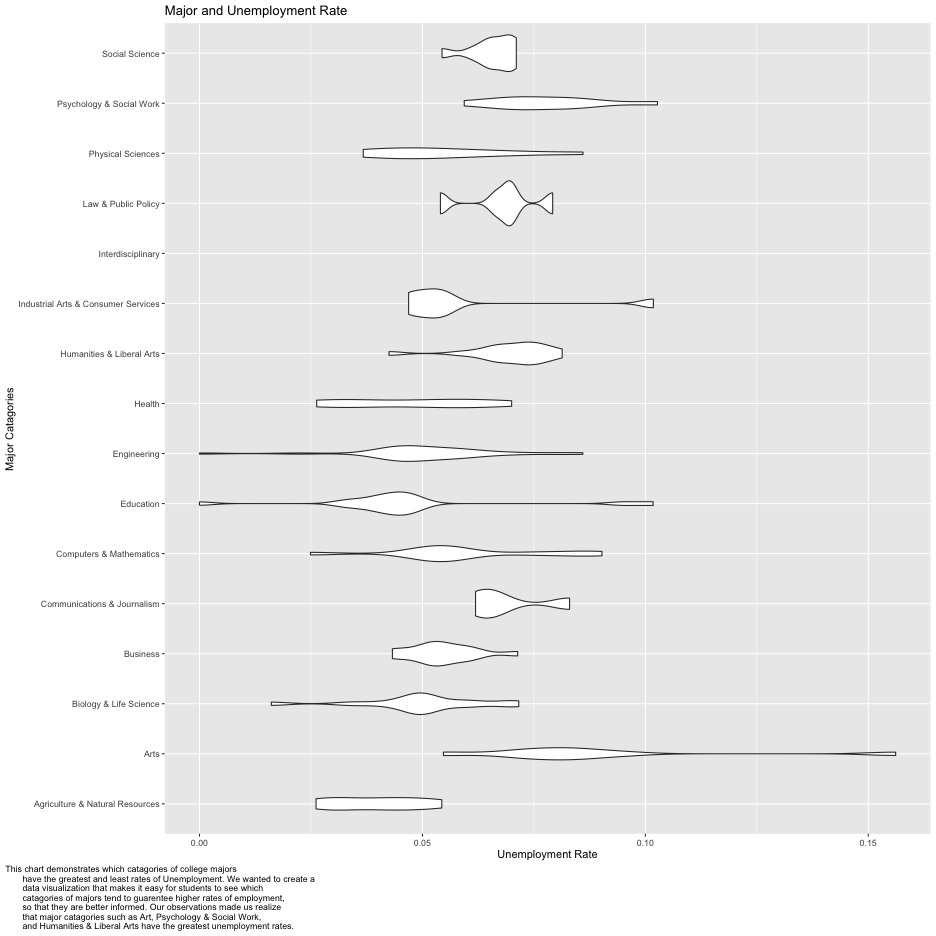
\includegraphics{index_files/figure-latex/all_ages_plot-1.pdf} This
chart demonstrates which categories of college majors have the greatest
and least rates of Unemployment. We wanted to create a data
visualization that makes it easy for students see which categories of
majors tend to guarantee higher rates of employment, so that they are
better informed. Our observations made us realize that major categories
such as Art, Psychology \& Social work and Humanities \& Liberal Arts
have the greatest unemployment rates.

\end{document}
